\input{../common}
\everymath{\displaystyle}
\begin{document}
  %<*content>
  \lesson{algebra}{10}{Schéma  de Bernoulli-  Loi binomiale}
  
 \subsection{Epreuve de Bernoulli}
  \begin{definition}
  Une  épreuve de Bernoulli  est une expérience aléatoire  qui ne comporte que deux issues, l'une appelée succès ($S$) et l'autre  échec ($\overline{S}$).
   
\end{definition}
\begin{example}
\begin{itemize}
\item On lance une pièce de monnaie équilibrée ou non. On appelle par exemple succès, l'issue Pile et échec, l'issue  Face.
\item  On lance un dé. On peut décider  d'appeler succès la sortie du 6 et échec la sortie de 1; 2; 3; 4   ou 5.

\end{itemize}
\end{example}
\subsection*{Loi de Bernoulli}
\begin{definition}
  Une  loi de Bernoulli  est  une loi de probabilité définie sur l'ensemble $ \Omega=\accol{S, \overline{S}} $ des issues d'une épreuve de Bernoulli.
  On associe  au succès $S$ la probabilité $ p $\; $ (0\leq p\leq 1)$.
  
   La probabilité de l'échec $ \overline{S} $  est donc $ 1-p $\\
  
  
   $\begin{array}{|c|c|c|c|c|}
\hline
 \text{Issue} &  S & \overline{S}    \\
 \hline
\text{probabilité} &  p &  1-p  \\
\hline
\end{array}$
 
  $ p $  est appelé le paramètre de la loi de Bernoulli.
  \end{definition}
  \begin{example}
  \begin{itemize}
 \item  On lance une pièce équilibrée. La probabilité du succès <<Obtenir Pile >> est $ p=\frac{1}{2} $.\\La loi de Bernoulli de paramètre $ \frac{1}{2} $  est donc:\\
 
   $\begin{array}{|c|c|c|c|c|}
\hline
\text{Issue} & \text{Pile} &\text{Face}  \\
 \hline
\text{probabilité} &  \frac{1}{2} &  \frac{1}{2}   \\
\hline
\end{array}$


\item  On lance un dé équilibré. La probabilité du succès <<Obtenir le 3 >> est $ p=\frac{1}{6} $.\\La loi de Bernoulli de paramètre $ \frac{1}{6} $  est  donc:\\
 $\begin{array}{|c|c|c|c|c|}
\hline
 \text{Issue} &  S & \overline{S}    \\
 \hline
\text{probabilité} &  \frac{1}{6} &  \frac{5}{6}   \\
\hline
\end{array}$
\end{itemize}
  \end{example}
   \subsection{Schéma de Bernoulli}
    \begin{definition}
 Un  schéma  de Bernoulli  est une répétition d'épreuves de Bernoulli identiques et indépendantes.
  \end{definition}
  \begin{remark}
  Des expériences aléatoires successives sont \textbf{indépendantes} lorsque l'issue de l'une quelconque de ces expériences  ne dépend pas de l'issue des autres.
  \end{remark}
  \begin{example}
 Une urne  contient 3 boules rouges et 1 boule verte. On tire successivement et avec remise 3 boules de l'urne.\\Pour chacun des tirages, l'évènement <<obtenir une boule verte>> est  considéré comme succès.
 
 
  On représente  à l'aide de l'arbre ci-dessous  les différents résultats.\\Les issues de cette répétition sont  des listes:$\;  (V,V,V);\quad (V,V,R); \quad (R,V,R);\quad (R,V,V)$...\\

 \begin{tikzpicture}[xscale=0.85,yscale=0.85]
 \draw (0,0)--(-2,0.5) node[midway, below, sloped]{$ \tfrac{3}{4} $};
 \draw (0,1)--(-2,0.5) node[midway, above, sloped]{$ \tfrac{1}{4} $};
 \draw (0,2)--(-2,2.5) node[midway, below, sloped]{$ \tfrac{3}{4} $};
 \draw (0,3)--(-2,2.5) node[midway, above, sloped]{$ \tfrac{1}{4} $};
 \draw (0,4)--(-2,4.5) node[midway, below, sloped]{$ \tfrac{3}{4} $};
 \draw (0,5)--(-2,4.5) node[midway, above, sloped]{$ \tfrac{1}{4} $};
 \draw (0,6)--(-2,6.5) node[midway, below, sloped]{$ \tfrac{3}{4} $};
 \draw (0,7)--(-2,6.5) node[midway, above, sloped]{$ \tfrac{1}{4} $};
 \draw (-2,0.5)--(-4,1.5) node[midway, below, sloped]{$ \tfrac{3}{4} $};
 \draw (-2,2.5)--(-4,1.5) node[midway, above, sloped]{$ \tfrac{1}{4} $};
 \draw (-2,4.5)--(-4,5.5) node[midway, below, sloped]{$ \tfrac{3}{4} $};
 \draw (-2,6.5)--(-4,5.5) node[midway, above, sloped]{$ \tfrac{1}{4} $};
 \draw (-4,1.5)--(-6,3.5) node[midway, below, sloped]{$ \tfrac{3}{4} $};
 \draw (-4,5.5)--(-6,3.5) node[midway, above, sloped]{$ \tfrac{1}{4} $};
 \draw (0,0) node[fill=white]{$R$};
 \draw (0,1) node[fill=white]{$V$};
 \draw (0,2) node[fill=white]{$R$};
 \draw (0,3) node[fill=white]{$V$};
 \draw (0,4) node[fill=white]{$R$};
 \draw (0,5) node[fill=white]{$V$};
 \draw (0,6) node[fill=white]{$R$};
 \draw (0,7) node[fill=white]{$V$};
 \draw (-2,0.5) node[fill=white]{$R$};
 \draw (-2,2.5) node[fill=white]{$V$};
 \draw (-2,4.5) node[fill=white]{$R$};
 \draw (-2,6.5) node[fill=white]{$V$};
 \draw (-4,1.5) node[fill=white]{$R$};
 \draw (-4,5.5) node[fill=white]{$V$};
 \end{tikzpicture}
  \end{example}
  \textbf{Remarque}:\; Si les tirages  ont lieu sans remise, il ne s'agit plus d'un schéma de Bernoulli car les expériences répétées ne sont plus identiques.
   \subsection{Loi binomiale}
  \begin{definition}
  On considère un schéma de Bernoulli, répétition de $ n $ épreuves de Bernoulli identiques et indépendantes de même paramètre  $ p $.  On note $ X $ la variable aléatoire qui associe à cette répétition de $ n $  épreuves, le nombre de succès.\\La loi de $ X $   est appelée \textbf{loi binomiale de paramètres  $ n$ et $ p$}.\\ On dit que $ X $  suit la loi binomiale $ \mathcal{B}(n, p) $.
    \end{definition}
   
    \begin{example}
On reprend l'exemple précédent et on note $ X $ la variable aléatoire égale au nombre de boules  vertes obtenues. $ X $  suit la loi binomiale $ \mathcal{B}(3,\tfrac{1}{4} ) $. Les valeurs possibles de $ X $  sont: $ 0;\;1;\;2;\;3 $ \; et \;$ 4 $\\
$ \bullet $ Calculons P$ (X=0 )$ \\Le nombre de chemins dans l’arbre réalisant  $ 0 $ succès parmi  $ 3 $ tirages est égal à $ 1. $ \; ( c'est $ C_{3}^{0}) $\\ Donc P$ (X=0 )=\paren{\tfrac{1}{4}}^{0}\times \paren{\tfrac{3}{4}}^{3}$\\
$ \bullet $ Calculons P$ (X=1 )$ \\Le nombre de chemins dans l’arbre réalisant  $ 1$ succès parmi  $ 3 $ tirages est égal à $ 3. $\; ( c'est $ C_{3}^{1}) $\\ Donc P$ (X=1 )=3\times\paren{\tfrac{1}{4}}^{1}\times \paren{\tfrac{3}{4}}^{2}$\\
$ \bullet $ Calculons P$ (X=2 )$ \\Le nombre de chemins dans l’arbre réalisant  $ 2$ succès parmi  $ 3 $ tirages est égal à $ 3. $\; ( c'est $ C_{3}^{2}) $\\ Donc P$ (X=2 )= 3\times\paren{\tfrac{1}{4}}^{2}\times \paren{\tfrac{3}{4}}^{1}$\\
$ \bullet $ Calculons P$ (X=3 )$ \\Le nombre de chemins dans l’arbre réalisant  $ 3$ succès parmi  $ 3 $ tirages est égal à $ 1. $\; ( c'est $ C_{3}^{3}) $\\ Donc P$ (X=1 )= 1\times\paren{\tfrac{1}{4}}^{3}\times \paren{\tfrac{3}{4}}^{0}$


La loi de $X$  est donc:\\
 
  

  $ \begin{array}{|c|c|c|c|c|}
\hline
  k  & 0 &1&2&3  \\
 \hline
P(X=k ) &  \frac{27}{64} &  \frac{27}{64}  & \frac{9}{64}  & \frac{1}{64} \\
\hline
\end{array}$
 
    \end{example}
\begin{remark}
 Le nombre de chemins dans l'arbre réalisant $ k $ succès  parmi $ n $ tirages est égal à  $ C_{n}^{k} $.
  \end{remark}

\begin{property}[Admis]
Si $ X $ est une variable aléatoire qui suit la loi binomiale de paramètres $ n$ et $ p$, alors pour entier $ k $ compris entre $ 0$ et $n $: $$ P(X=k)=C_{n}^{k}p^{k}(1-p)^{n-k} $$
  \end{property} 
  \begin{property}[Admis]
 Si $ X $ est une variable aléatoire qui suit la loi binomiale de paramètres $ n$ et $ p$, alors:
\[\bullet\;\; \text{E(X)=}np \hspace*{2cm} \bullet \;\;\text{V(X)}=np(1-p)\]
\end{property} 

\begin{exercice}
   Un QCM  comporte trois questions. Pour chacune d'elles, quatre réponses sont proposées dont une seule est correcte. Un élève donne au hasard une réponse à chaque question. On note $ X $ le nombre de réponses correctes données par l'élève.
   \begin{enumerate}
   \item Justifier que la situation relève d'une loi binomiale dont on précisera les paramètres.
   \item  Déterminer la loi de probabilité de la variable aléatoire $ X. $
   \item Calculer E(X)  et $\sigma(X)  $.
   \end{enumerate}
\end{exercice}
\begin{proof}
  \begin{enumerate}
  \item Choisir au hasard une réponse à une question peut-être considéré  comme une épreuve de Bernoulli.  On appelle succès le choix de la réponse correcte; sa probabilité est $ p=\frac{1}{4} $.\\ il y a  donc une répétition de trois épreuves identiques et indépendantes.L'expérience   décrite est bien un schéma  de Bernoulli. La variable aléatoire qui prend le nombre de succès c-à-d le nombre de bonnes réponses données par l'élève, suit la loi binomiale  de paramètres $3$ et $ \frac{1}{4}$.
  \item La variable aléatoire $ X$   prend les valeurs 0; 1; 2 ou 3.\\
  P($ X=0)=C_{3}^{0}\paren{\frac{1}{4}}^{0}\paren{\frac{3}{4}}^{3}= \frac{27}{64}$\\
   P($ X=1)=C_{3}^{1}\paren{\frac{1}{4}}^{1}\paren{\frac{3}{4}}^{2}= \frac{27}{64}$\\
    P($ X=2)=C_{3}^{2}\paren{\frac{1}{4}}^{2}\paren{\frac{3}{4}}^{1}= \frac{9}{64}$\\
     P($ X=3)=C_{3}^{3}\paren{\frac{1}{4}}^{3}\paren{\frac{3}{4}}^{0}= \frac{1}{64}$\\
 
  
  $ \begin{array}{|c|c|c|c|c|}
\hline
  k  & 0 &1&2&3  \\
 \hline
P(X=k ) &  \frac{27}{64} &  \frac{27}{64}  & \frac{9}{64}  & \frac{1}{64}  \\
\hline
\end{array}$
\item $ X $  suit la loi binomiale  de paramètres $3$ et $ \frac{1}{4}$ donc:\\
E(X)$ =3\times \frac{1}{4}=\frac{3}{4} \quad \quad$, V(X)$ =3\times \frac{1}{4}\times\frac{3}{4}=\frac{9}{16}\quad $ et $\quad \sigma(X)=\frac{3}{4} $.
 \end{enumerate}
 Si un grand nombre de personnes répondent au hasard à ce QCM, alors on observera en moyenne 0.75 bonne réponse par QCM.
 \end{proof}
  %</content>
\end{document}
